%Notes by Harsh Mistry 
%CS 349
%Based on Template From  https://www.cs.cmu.edu/~ggordon/10725-F12/template.tex

\documentclass[twoside]{article}
\setlength{\oddsidemargin}{0.25 in}
\setlength{\evensidemargin}{-0.25 in}
\setlength{\topmargin}{-0.6 in}
\setlength{\textwidth}{6.5 in}
\setlength{\textheight}{8.5 in}
\setlength{\headsep}{0.75 in}
\setlength{\parindent}{0 in}
\setlength{\parskip}{0.1 in}
\usepackage{amsmath,amsfonts,graphicx}
\newcounter{lecnum}
\renewcommand{\thepage}{\thelecnum-\arabic{page}}
\renewcommand{\thesection}{\thelecnum.\arabic{section}}
\renewcommand{\theequation}{\thelecnum.\arabic{equation}}
\renewcommand{\thefigure}{\thelecnum.\arabic{figure}}
\renewcommand{\thetable}{\thelecnum.\arabic{table}}
\newcommand{\lecture}[4]{
   \pagestyle{myheadings}
   \thispagestyle{plain}
   \newpage
   \setcounter{lecnum}{#1}
   \setcounter{page}{1}
   
   
%Info Box 
   \begin{center}
   \framebox{
      \vbox{\vspace{2mm}
    \hbox to 6.28in { {\bf CS 349 - User Interfaces
	\hfill Winter 2018} }
       \vspace{4mm}
       \hbox to 6.28in { {\Large \hfill Lecture #1: #2  \hfill} }
       \vspace{2mm}
       \hbox to 6.28in { {\it Lecturer: #3 \hfill Notes By: #4} }
      \vspace{2mm}}
   }
   \end{center}
   
   \markboth{Lecture #1: #2}{Lecture #1: #2}



 
}

\renewcommand{\cite}[1]{[#1]}
\def\beginrefs{\begin{list}%
        {[\arabic{equation}]}{\usecounter{equation}
         \setlength{\leftmargin}{2.0truecm}\setlength{\labelsep}{0.4truecm}%
         \setlength{\labelwidth}{1.6truecm}}}
\def\endrefs{\end{list}}
\def\bibentry#1{\item[\hbox{[#1]}]}

\newcommand{\fig}[3]{
			\vspace{#2}
			\begin{center}
			Figure \thelecnum.#1:~#3
			\end{center}
	}
	
\graphicspath{ {images/} }

\newtheorem{theorem}{Theorem}[lecnum]
\newtheorem{lemma}[theorem]{Lemma}
\newtheorem{ex}[theorem]{Example}
\newtheorem{proposition}[theorem]{Proposition}
\newtheorem{claim}[theorem]{Claim}
\newtheorem{corollary}[theorem]{Corollary}
\newtheorem{definition}[theorem]{Definition}
\newenvironment{proof}{{\bf Proof:}}{\hfill\rule{2mm}{2mm}}
\newcommand\E{\mathbb{E}}


%Start of Document 
\begin{document}

\lecture{4}{January 10, 2018}{Keiko Katsuragawa}{Harsh Mistry}

\section{Drawing}

\subsection{Drawing Primitives}
\begin{itemize}
\item Pixel \\
\verb|SetPixel(x,y. c)|\\
\verb|DrawImage(x,y,w,h,img)|
\item Stoke \\
\verb|DrawLine(x1, y1, x2, y2, colour)|\\
\verb|DrawRect(x,y , w, h, colour)|\\
\item Region\\
\verb|DrawText("A", x, y, colour)|\\
\verb|DrawRect(x, y, w, h, colour, thick, fill)|
\end{itemize}

\subsection{Graphics Context}
\begin{itemize}
\item Gather all options into a structure, pass it to teh draw routines
\item In X, the graphics context is stored on hthe X server
\item Modern systems like Java and Open GL have graphics context 
\begin{itemize}
\item Java : Graphics Object
\item OpenGL : Attribute State
\end{itemize}
\end{itemize}

\begin{center}
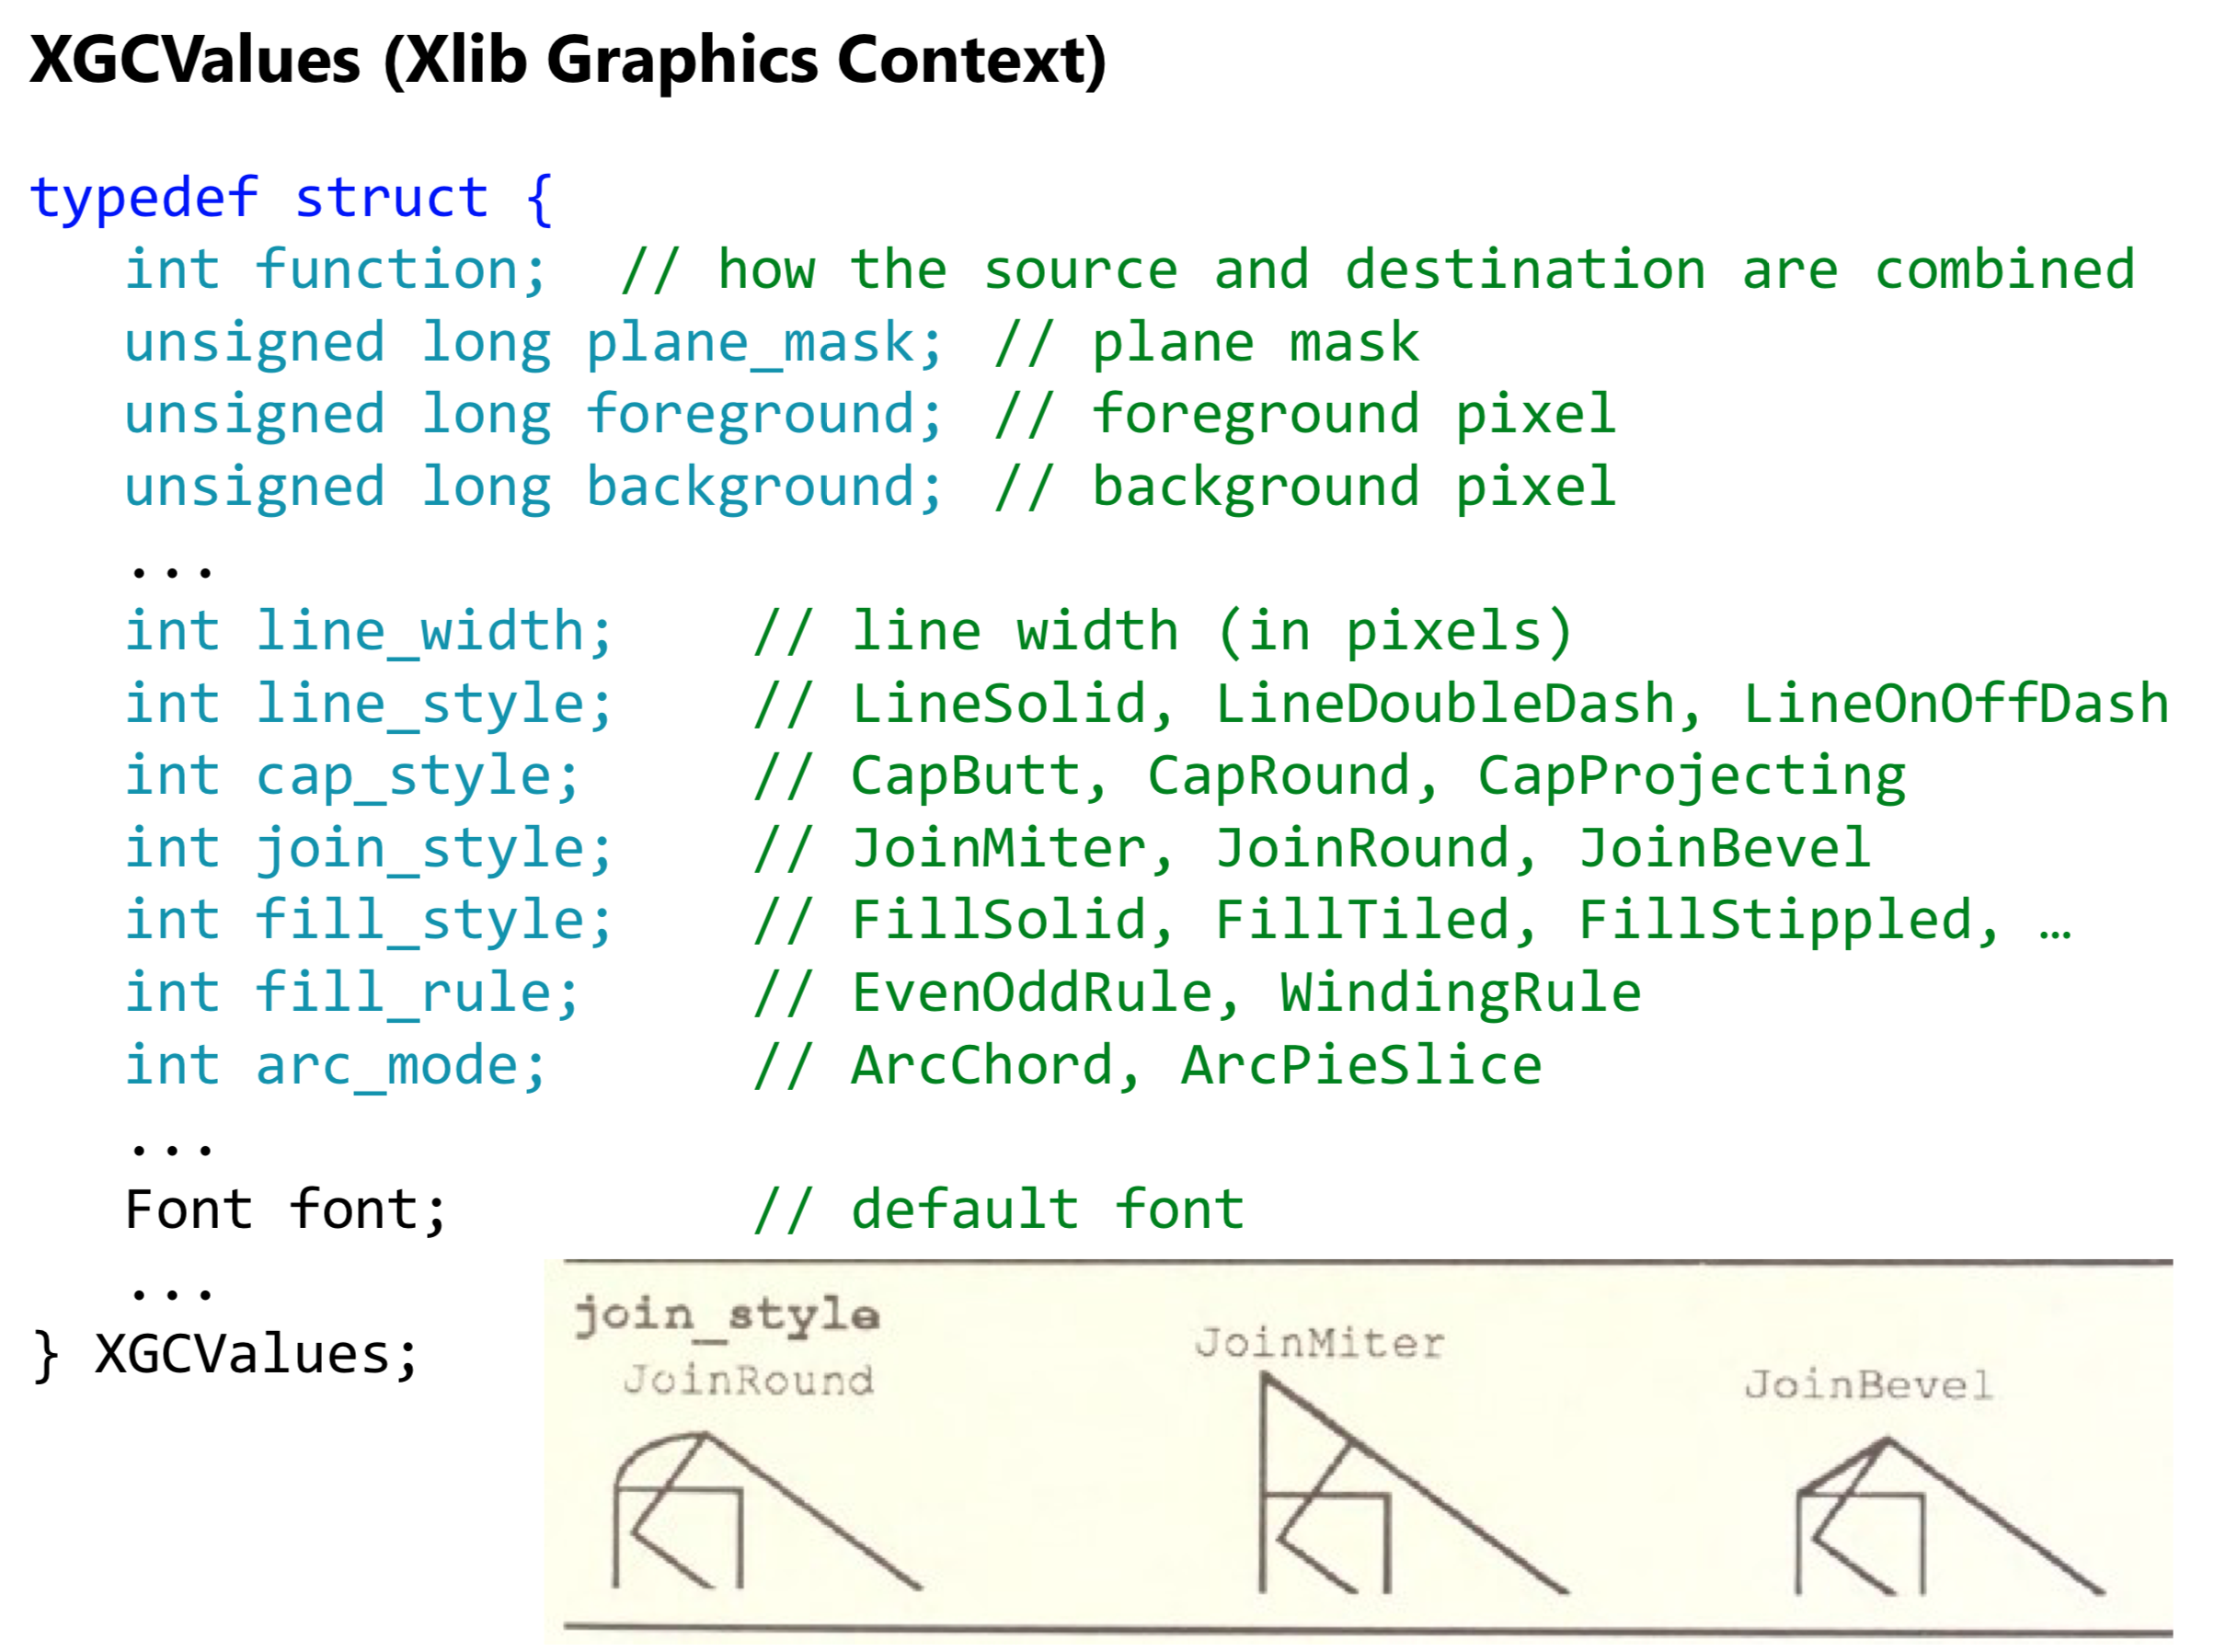
\includegraphics[scale=0.2]{4}\\
Taken From Class Slides
\end{center}

\subsection{Painter Algorithm}
\begin{itemize}
\item Basic graphics primitives are (really) primitive
\item To draw more complex shapes : 
\begin{itemize}
\item Combine primitives
\item Draw back-to-front, layering the image
\end{itemize}
\end{itemize}

\begin{center}
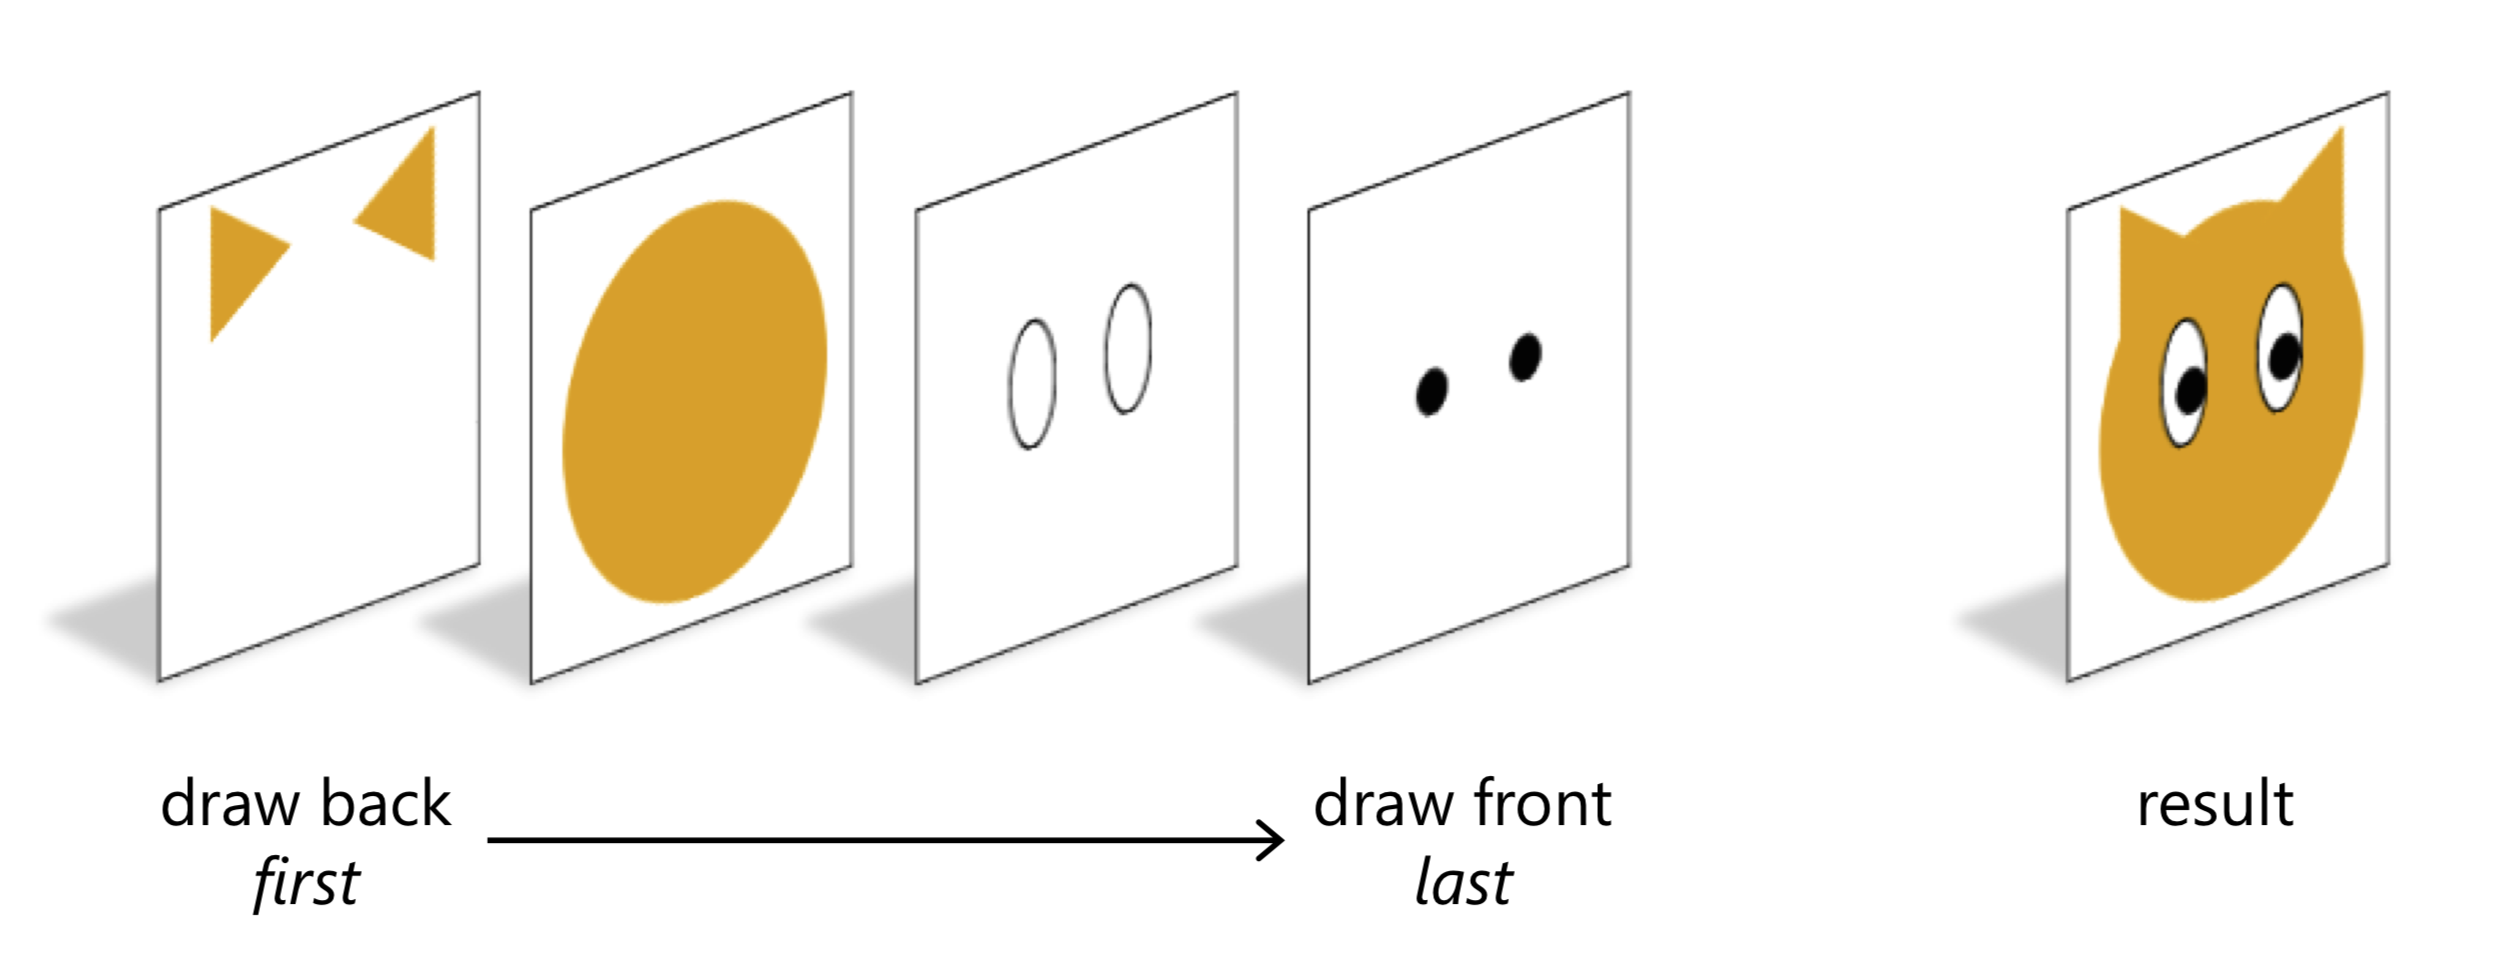
\includegraphics[scale=0.2]{5}\\
Taken From Class Slides
\end{center}

\subsubsection{Implementing Painters Algorithm}
\begin{itemize}
\item Think about things your program needs to paint 
\item Package drawing of each thing into a n object that can draw itself
\begin{itemize}
\item Implement a Displayable base class with virtual "paint" method 
\item Derive classes for the things you want to display
\end{itemize}
\item Keep an ordered display list of displayable objects
\item To repaint
\begin{itemize}
\item Clear the screen 
\item Repain everything in the display list. 
\end{itemize}
\end{itemize}

\end{document}





